\documentclass[a4paper]{abnt}

%% Acentos
\usepackage[utf8]{inputenc}

%% - Abnt UFPR -
\usepackage{abnt-UFPR}
\usepackage[num]{abntcite}

%% - Outros Pacotes -
\usepackage{here}
\usepackage{url}
\usepackage{amsmath}
\usepackage{graphicx}
% Python listing setup

\usepackage{color}
\usepackage{listings}
\usepackage{textcomp}
\usepackage{setspace}
\usepackage{palatino}

\renewcommand{\lstlistlistingname}{Code Listings}
\renewcommand{\lstlistingname}{Code Listing}
\definecolor{gray}{gray}{0.5}
\definecolor{green}{rgb}{0,0.5,0}

\lstnewenvironment{python}[1][]{
\lstset{
language=python,
basicstyle=\ttfamily\small\setstretch{1},
stringstyle=\color{red},
showstringspaces=false,
alsoletter={1234567890},
otherkeywords={\ , \}, \{},
keywordstyle=\color{blue},
emph={access,and,break,class,continue,def,del,elif,else,%
except,exec,finally,for,from,global,if,import,in,is,%
lambda,not,or,pass,print,raise,return,try,while},
emphstyle=\color{black}\bfseries,
emph={[2]True, False, None, self},
emphstyle=[2]\color{green},
emph={[3]from, import, as},
emphstyle=[3]\color{blue},
upquote=true,
morecomment=[s]{"""}{"""},
commentstyle=\color{gray}\slshape,
emph={[4]1, 2, 3, 4, 5, 6, 7, 8, 9, 0},
emphstyle=[4]\color{blue},
literate=*{:}{{\textcolor{blue}:}}{1}%
	{=}{{\textcolor{blue}=}}{1}%
	{-}{{\textcolor{blue}-}}{1}%
	{+}{{\textcolor{blue}+}}{1}%
	{*}{{\textcolor{blue}*}}{1}%
	{!}{{\textcolor{blue}!}}{1}%
	{(}{{\textcolor{blue}(}}{1}%
	{)}{{\textcolor{blue})}}{1}%
	{[}{{\textcolor{blue}[}}{1}%
	{]}{{\textcolor{blue}]}}{1}%
	{<}{{\textcolor{blue}<}}{1}%
	{>}{{\textcolor{blue}>}}{1},%
frame=single
}}{}

\usepackage[tight,raggedright]{subfigure}
\usepackage[left=2cm,top=2.5cm,right=2cm,bottom=2cm]{geometry}
\usepackage[brazil]{babel}

\sloppy
\tolerance=9999999
\graphicspath{{img/}}

% -----------------------------------------------------------------------
\begin{document}

\autor{Jonatas Teixera\\Luan Haddad Ricardo dos Santos}
\titulo{Um editor de grafos para simulação de algoritmos}
\orientador{Alexandre Ibrahim Direne}

\comentario{Trabalho de conclusão de curso apresentado para obtenção do Grau 
de Bacharel em Ciência da Computação pela Universidade Federal do Paraná.}
\instituicao{Departamento de Informática \par Universidade Federal do Paraná}
\local{Curitiba - PR, Brasil}
\data{27 de dezembro de 2011}

\capa
\folhaderosto

\chapter*{Agradecimentos}
Somos gratos aos nossos pais, Fabio Ricardo dos Santos, Christina Bady Haddad Ricardo dos Santos e Attilio Teixeira Junior, Mariluz Teixeira, que foram os grandes patrocinadores da nossa graduação. Agradecemos também aos nossos amigos: Anderson, Andrio, Danilo, Derik, Diego, Felipe, Fernando e Raphael, alguns por terem estado junto de nós em projetos na universidade, outros por terem partilhado de bons momentos acadêmicos. Não podemos deixar de lembrar ao bom e velho labJoe, o qual sem ele esse trabalho não seria possível. Gostaríamos de lembrar o nome do nosso orientador Alexandre Ibrahim Direne que aceitou nos orientar na execução deste trabalho. Além disto agradecemos à Kauana de Oliveira Grola, namorada do Luan pelo apoio moral.

% -----------------------------------------------------------------------
\pagenumbering{roman}
\setcounter{page}{1}
\sumario
\listadefiguras
\listadetabelas

% -----------------------------------------------------------------------
\begin{resumo}
Esse trabalho tem a intenção de mostrar o funcionamento e a utilização do Grape que é uma ferramenta para edição de grafos e simulação de algoritmos. O Grape fornece uma interface de autoria para implementação de algoritmos e os executa de maneira gráfica através de passos iterativos, os quais facilitam a construção, compreensão e depuração dos algoritmos, dispõe de uma interface personalizável para diferentes representações dos grafos. Esta ferramenta foi projetada sendo multiplataforma, e seus algoritmos podem ser incluídos facilmente sem a necessidade de recompilações. Aqui será apresentado um breve resumo a respeito de teoria dos grafos, para que haja familiaridade com os termos e para que demais detalhes do grape possam ser expostos. 

\noindent \textbf{Palavras-chave}: Grafos, editor de grafos, algoritmos, simulador.
\end{resumo}

% -----------------------------------------------------------------------
\chapter{Introdução}
\setcounter{page}{10}
Durante as disciplinas de grafos e inteligência artificial ministrados no curso de graduação percebemos a carência de representações visuais de determinadas estruturas de dados, para tal fim iniciamos a implementação do Grape, que sugere uma alternativa similar ao que é comumente visto em sala de aula, onde o professor representa grafos e árvores com nós representados com pequenas esferas com algum identificador, e arestas que ligam esses nós seguindo uma lógica qualquer. 

Por grafo ser um modelo matemático mais abrangente, este foi escolhido para ser abordado neste trabalho. Após a necessidade de utilizar a ferramenta GRAFO \cite{grafo} na disciplina de algoritmos e teoria dos grafos enfrentamos algumas limitações, como não ser possível a confecção de multi-grafos, di-grafos e multi-di-grafos, não haver a possibilidade de adição de diferentes atributos a cada vértice ou aresta assim como a seleção de múltiplos vértices e ainda a abertura de vários grafos simultaneamente em abas ou janelas. 

Apesar de grande interesse na ferramenta após uma análise da possibilidade de continuar o GRAFO,  percebemos que a estrutura de dados interna causaria alguns problemas na representação de multi-grafos e a reestruturação da interface seria algo demasiadamente trabalhoso, então aproveitamos a oportunidade para introduzir novas ferramentas tecnológicas e iniciar a implementação do Grape.
% -----------------------------------------------------------------------
\chapter{Teoria dos Grafos}
\label{sec:revisao_bibliografica}
A origem da teoria dos grafos se deu a partir do problema ocorrido na cidade Königsberg aonde a população desejava saber como atravessar as sete pontes da cidade sem que a mesma ponte fosse atravessada mais de uma vez. Este problema foi estudado pelo matemático Euler que provou não haver solução.

\begin{figure}[htb]
    \centering
	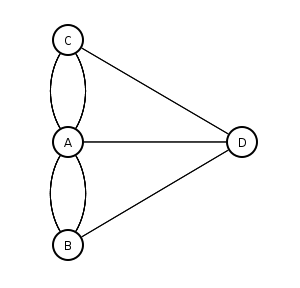
\includegraphics[width=6cm]{euler_graph.png}
	\caption{Grafo de Euler}
	\label{img_graph_euler}
\end{figure}

Para simplificar o problema Euler ignorou alguns aspectos como largura dos rios e forma das ilhas e continentes, mantendo apenas a existência ou não de conexões entre dois pontos da cidade. Esse novo campo da matemática se tornou uma ferramenta importante para analisar problemas reais. Para compreender um pouco melhor vamos definir um grafo \textbf{G} sendo um par ordenado \textbf{$G = (V, E)$} tal que:

\begin{itemize}
    \item \textbf{V} é um conjunto não vazio de \textbf{vértices} ou nodos.
    \item \textbf{E} é um conjunto de \textbf{arestas} ou arcos que por sua vez são pares de vértices distintos.
\end{itemize}

Quando dois vértices são conectados por uma aresta, estes são chamados de \textbf{adjacentes}. O \textbf{grau} de um vértice é o número de arestas que terminam no vértice, um vértice é chamado \textbf{pendant} quando o seu grau é um.

Um grafo é chamado \textbf{multi-grafo} quando existem mais de uma aresta conectando o mesmo par de vértices, e um grafo é completo quando para todos pares de vértices existe pelo menos uma aresta conectando-os, denota-se Kn um grafo completo com n vértices, como podemos ver na figura \ref{img_complete_graphs} um exemplo de grafo \textbf{completo} com $n <= 6$

\begin{figure}[htb]
    \centering
	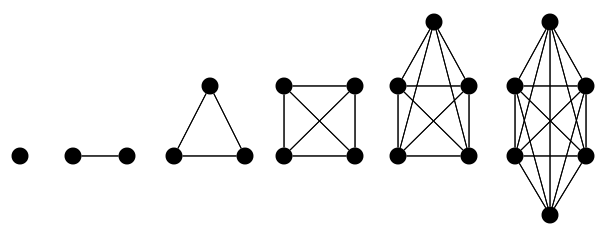
\includegraphics[width=12cm]{complete_graphs.png}
	\caption{Grafos completos}
	\label{img_complete_graphs}
\end{figure}

Além dos grafos comuns, podemos ter \texbf{grafos dirigidos} ou \texbf{digrafos}, nestes grafos as arestas tem direção, ou seja, saem de um vértice e chegam a outro, sem necessariamente ter volta. Nos di-grafos o grau é muitas vezes dividido em \texbf{grau de entrada} e \texbf{grau de saída}, quantidade de arestas que chegam e que saem do vértice, respectivamente. Chamamos uma sequência de arestas em um grafo de caminho e o tamanho do \texbf{caminho} é dado pelo número de arestas nesta sequência.

\begin{figure}[htb]
    \centering
	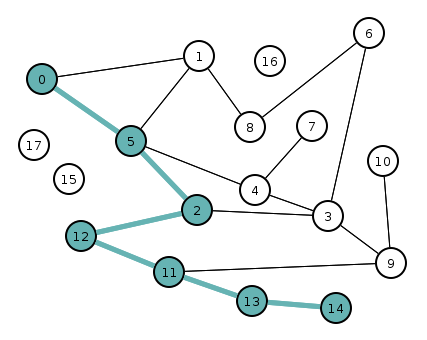
\includegraphics[width=10cm]{path.png}
	\caption{Caminho}
	\label{img_path}
\end{figure}

Um caminho é uma sequência de arestas consecutivas em um grafo e o tamanho do caminho é o número de arestas atravessadas. A figura \ref{img_path} demonstra um caminho em um grafo com início no vértice 0 e fim no vértice 14.

Um circuito ou \textbf{ciclo} é um caminho que tem inicio e fim no mesmo vértice, a ilustração na figura \ref{img_cilce} representa um ciclo em um grafo, um laço é um ciclo de tamanho um, ou seja, uma aresta que conecta um vértice a ele mesmo, grafos que possuem \texbf{laços} são chamados e \texbf{pseudografos}.

\begin{figure}[htb]
    \centering
	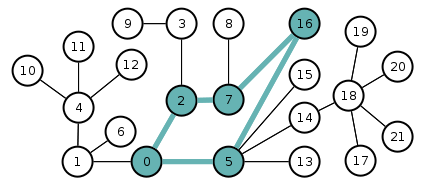
\includegraphics[width=10cm]{cicle.png}
	\caption{Ciclo}
	\label{img_cilce}
\end{figure}

Um grafo onde existe pelo menos um caminho conectando todo par de vértice é chamado de grafo \texbf{conexo}, caso um grafo não seja conexo, é possível dividi-lo em \textbf{componentes conexas}, que são subgrafos conexos disjuntos, como pode ser visto na figura \ref{img_component}.

\begin{figure}[htb]
    \centering
	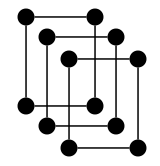
\includegraphics[width=5cm]{component.png}
	\caption{Grafo com três componentes conexas}
	\label{img_component}
\end{figure}

Chamamos de \texbf{vértice de corte} ou \texbf{ponto de articulação} um vértice que se removido do grafo, produz um novo grafo com mais componentes conexas que anteriormente.

Um \texbf{grafo planar} é um grafo que pode ser representado no plano de tal forma que suas arestas não se cruzem. Segundo o Teorema de Kuratowski \cite{kuratowski}, um grafo planar não pode apresentar nem o grafo completo K5 nem o grafo bipartido K3,3 como subgrafos.

O problema explicado anteriormente das sete pontes da cidade de Königsberg ficou conhecido como caminho de Euler, ou seja, um Caminho Euleriano é um caminho em um grafo que visita cada aresta sem que a mesma seja revisitada, em casos especiais um Circuito Euleriano é um caminho Euleriano que começa e termina no mesmo vértice, dessarte, grafos que possuem um circuito Euleriano são chamados Grafos Eulerianos. 

O matemático Willian Hamilton \cite{hamilton} criou o jogo icosiano na época da Guerra Civil Americana que consistia em um dodecaedro sólido que forma um grafo planar de vinte vértices e trinta arestas onde cada vértice representa uma cidade (figura \ref{img_icosian}).

\begin{figure}[htb]
    \centering
	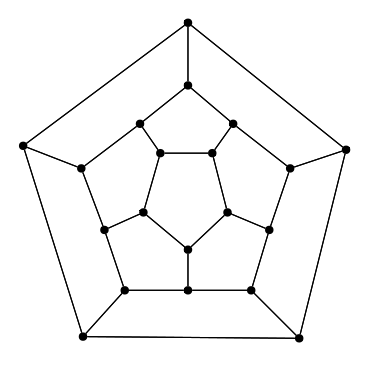
\includegraphics[width=6cm]{icosian.png}
	\caption{Grafo jogo icosiano}
	\label{img_icosian}
\end{figure}

Este jogo tem como objetivo passar por todas as cidades uma única vez sendo que o percurso deve iniciar e terminar no mesmo vértice, formando um circuito que recebeu o nome de \textbf{circuito Hamiltoniano}. Em outras palavras um caminho Hamiltoniano é um caminho que passa por todos os vértices uma única vez, e um circuito Hamiltoniano é um caminho Hamiltoniano que inicia e termina no mesmo vértice.

\begin{figure}[htb]
    \centering
	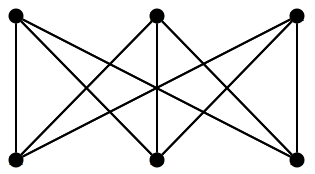
\includegraphics[width=6cm]{k33.png}
	\caption{Grafo bipartido completo (K3,3)}
	\label{img_k33}
\end{figure}

Chamamos um grafo de bipartido quando seus vértices podem ser divididos em dois subconjuntos U e V.  Cada aresta conecta um vértice de U a um vértice de V, nunca um vértice de V a outro de V ou de um vértice de U a outro de U.\\Grafo bipartido completo é um grafo bipartido onde todos os vértices do subconjunto U são adjacentes a todos os vértices do conjunto V (figura \ref{img_k33}).
O número cromático de um grafo é o menor número de cores que são necessárias para colorir todos os vértices de modo que nenhum vértice adjacente tenha a mesma cor. Todo grafo planar pode ser colorido com no máximo quatro cores, essa propriedade chamasse Teorema das quatro cores, e podemos ver um exemplo disso na figura \ref{img_graph_color}.

\begin{figure}[htb]
    \centering
	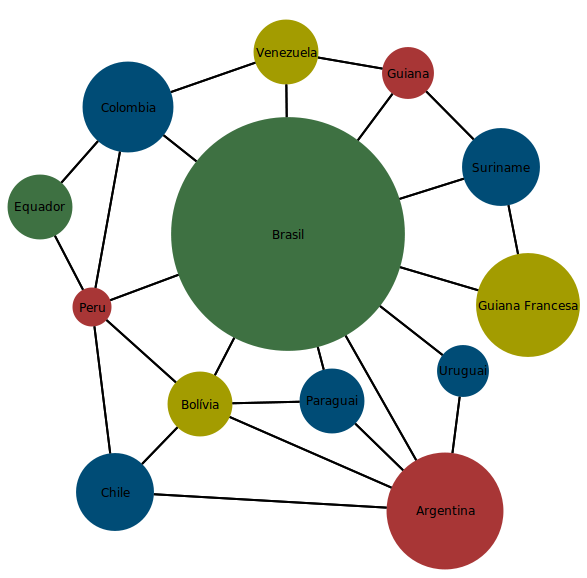
\includegraphics[width=12cm]{graph_color.png}
	\caption{Grafo dos países e fronteiras da América do Sul}
	\label{img_graph_color}
\end{figure}

% -----------------------------------------------------------------------
\chapter{Estrutura de dados}
Como já foi discutido neste trabalho um grafo é um modelo matemático, e para este modelo existem algumas alternativas de representações computacionais, tais como matrizes e listas de adjacência.

\begin{figure}[htb]
    \centering
	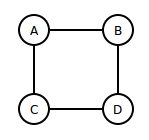
\includegraphics[width=5cm]{graph_sample.png}
	\caption{Exemplo de grafo}
	\label{img_graph_sample}
\end{figure}

\section{Matriz de adjacência}
Para um grafo G com n vértices, podemos representá-lo em uma matriz $A_{n x n}$, onde cada entrada da matriz pode ser definida de acordo com as propriedades do grafo a ser representado, porém é comum o valor $a_{ij}$ conter a informação de como os vértices se relacionam. Isto é, para representar um grafo não direcionado simples e sem pesos podemos simplesmente assumir que em cada entrada tenha 1 ou 0, tal que 1 representa a existência da conexão entre os vértices e 0 que a mesma não há. Em outras palavras, representa a presença ou não de uma aresta.
Por exemplo a tabela \ref{tab_adj_matrix} é uma matriz $5 x 5$ que representa o grafo da figura \ref{img_graph_sample}.

\begin{table}[H]
        \centering
        \begin{tabular}{|l||c|c|c|c|} \hline
		---         & \textbf{A} & \textbf{B} & \textbf{C} & \textbf{D} \\ \hline \hline
		\textbf{A}  & 0          & 1          & 1          & 0 \\ \hline
		\textbf{B}	& 1          & 0          & 0          & 1 \\ \hline
		\textbf{C}	& 1          & 0          & 0          & 1 \\ \hline
		\textbf{D}	& 0          & 1          & 1          & 0 \\ \hline
        \end{tabular}
        \caption{Matriz de adjacência do grafo representado na figura \ref{img_graph_sample}.}
\label{tab_adj_matrix}
\end{table}

\section{Lista de adjacência}
Uma lista de adjacência (estrutura de adjacência ou dicionário) é a representação das arestas de um grafo em uma lista. Em outras palavras, cada vértice contem uma lista de adjacência a qual representa os vértices vizinhos deste.

O grafo da figura \ref{img_graph_sample} pode ser representado pela seguinte estrutura demonstrada na tabela \ref{tab_adj_list}

\begin{table}[H]
        \centering
        \begin{tabular}{|l|c|c|} \hline
		\textbf{A}  & adjacente a   & [\textbf{B}, \textbf{C}] \\ \hline \hline
		\textbf{B}	& adjacente a   & [\textbf{A}, \textbf{D}] \\ \hline \hline
		\textbf{C}	& adjacente a   & [\textbf{A}, \textbf{D}] \\ \hline \hline
		\textbf{D}	& adjacente a   & [\textbf{B}, \textbf{C}] \\ \hline
        \end{tabular}
        \caption{Lista de adjacência do grafo representado na figura \ref{img_graph_sample}.}
\label{tab_adj_list}
\end{table}
Para uma representação utilizando listas de adjacência, nós devemos manter para cada vértices uma lista de todos os outros vértices com os quais ele tem aresta.

Um contra desta estrutura é não haver um lugar para manter informações relativas à aresta, como por exemplo peso, cumprimento, cor ou custo.

\section{Lista de incidência}
Percebendo que em uma Matriz de adjacência apesar de haver a possibilidade de manter uma informação referente à aresta ainda existem muitas limitações para armazenamento de informações referentes a cada vértice. Por outro lado, na representação de Lista de adjacência é possível armazenamento de informações em cada vértice, porém não existem a possibilidade de representar demais informações para as arestas. Tal abordagem é defendida em alguns textos como o de Goodrich e Tamassia em \cite{tamassia} e \cite{goodrich}.

\section{Representação no Grape}
Como no Grape, precisamos que cada vértice e aresta tenham os seus próprios atributos, utilizamos uma abordagem orientada a objetos e descrevemos uma estrutura de dados onde temos uma classe nomeada Vertex para os vértices e outra Edge para as arestas.

Um objeto Vertex tem uma lista de objetos Edge e cada objeto Edge mantem um ponteiro para os vértices de de início em fim que para grafos direcionados dão noção de direção às arestas.

Com uma abordagem orientada a objetos existe a possibilidade de armazenar mais informações para as arestas e vértices, como por exemplo: peso, cor, etc. Como no Grape existe a grande preocupação com a representação gráfica deste grafo, é dentro dessas classes o lugar propício para manter tais informações, como tamanho, espessura, posição e demais informações gráficas.
\begin{figure}[htb]
    \centering
	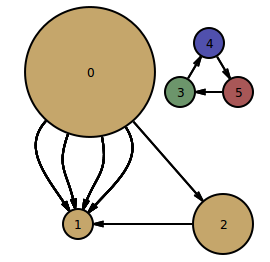
\includegraphics[width=5cm]{graph_struct.png}
	\caption{Exemplo de possibilidade de edição do grafo}
	\label{img_graph_struct}
\end{figure}

\chapter{Interface}
Neste capítulo iremos detalhar a interface do Grape, tais como menus, atalhos, opções, ferramentas, configurações, logs, e todas as outras maneiras de interagir com o usuário. Será apresenta do a barra de menus, ferramentas, divisão e múltipla edição distribuída em abas, e área de pintura.

Nota: O Grape é multi-plataforma, isto é, sua interface pode conter leves divergências ao que esta sendo mostrado de acordo com o sistema em que esta sendo executado. Neste trabalho iremos demonstrar o software usando Linux.

\section{Barra de menus}
A barra de menu é responsável por gerenciar entradas e saídas, configuração do ambiente do Grape, edição do grafo, edição do que deve ou não ser mostrado na tela, execução de algorítimos e créditos.
\begin{figure}[htb]
    \centering
	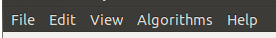
\includegraphics[width=5cm]{grape_menu.png}
	\caption{Menu}
	\label{img_grape_menu}
\end{figure}

\subsection{Menu File (Arquivo)}
\begin{figure}[htb]
    \centering
	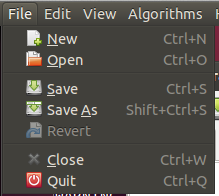
\includegraphics[width=5cm]{grape_menu_file.png}
	\caption{Menu arquivo}
	\label{img_grape_menu_file}
\end{figure}

No menu do arquivo existem opções de entra e saída do Grape, ou seja, possibilidade abrir, salvar, fechar, reverter para ultima versão salva, sair; ver figura \ref{img_grape_menu_file}
\begin{itemize}
    \item \textbf{New (Novo)}: Fornece a possibilidade de criar um novo grafo, inicialmente vazio.
    \item \textbf{Open (Abrir)}: Esta opção permite que um grafo criado no Grape seja aberto novamente, permitindo re-edições.
    \item \textbf{Save (Salvar)}: Opção responsável por salvar o grafo aberto na aba atual, em um local a ser especificado posteriormente ao usuário. (figura \ref{img_grape_menu_file})
    \item \textbf{Save As (Salvar Como)}: Esta opção permite que um arquivo que já tenha sido salvo anteriormente possa ser re-escrito em um caminho diferente, mantendo uma cópia no local anterior.
    \item \textbf{Revert (Reverter)}: Descarta todas as ações efetuadas no grafo, e retorna o seu estado para o mesmo que está salvo em disco.
    \item \textbf{Close (Fechar)}: Fecha a aba atual. Caso o grafo não tenha sido salvo, um diálogo irá aparecer para auxiliar nesta tarefa.
    \item \textbf{Quit (Sair)}: Essa ação irá fechar todas as abas e encerrar o grape, salvando os seus logs e suas configurações.
\end{itemize}

\begin{figure}[htb]
    \centering
	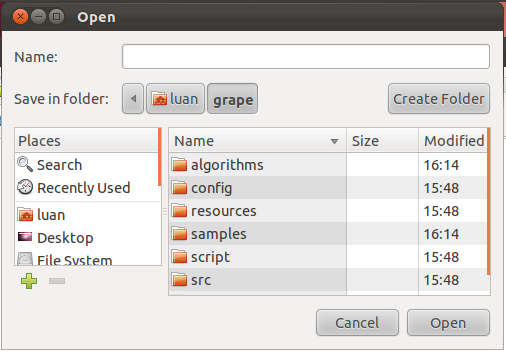
\includegraphics[width=10cm]{open_dialog.png}
	\caption{Abrir arquivo}
	\label{img_open_dialog}
\end{figure}

\subsection{Menu Edit (Editar)}

Esse menu é responsável por todas as ações de manipulação do grafo, e preferências globais. Todas a edições e modificações afetaram o grafo da aba que estiver com foco, com exceção da opção Preferências que irá atualizar as preferências globais do Grape.
\begin{figure}[htb]
    \centering
	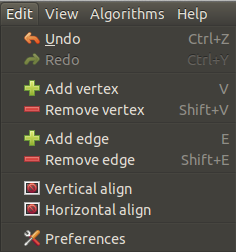
\includegraphics[width=6cm]{grape_menu_edit.png}
	\caption{Menu editar}
	\label{img_menu_edit}
\end{figure}

\begin{itemize}
    \item \textbf{Undo (Desfazer)}: Toda ação efetuada em cima de um grafo é salva em um pilha de ações, para que possa ser desfeita em caso de acidentes. A ação desfazer, desfaz a ultima ação.
    \item \textbf{Redo (Refazer)}: Essa ação refaz uma ação desfeita com o Desfazer.
    \item \textbf{Add Vertex (Adicionar Vértice)}: Habilita o modo de adição de vértices, em outras palavras, um vértice será criado assim que houver um clique com o botão esquerdo do mouse na área de pintura.
    \item \textbf{Remove Vertex (Remover Vértice)}: Remove o/os vértices que estejam selecionados e todas as arestas que tenham alguma conexão com os estes.
    \item \textbf{Add Edge (Adicionar Aresta)}: Quando esta opção for acionada, caso haja somente um vértice selecionado surgirá uma “aresta” tracejada entre o vértice selecionando e o ponteiro do mouse, desde que este esteja sobre a área de pintura, então será necessário que o usuário clique sobre um segundo vértice para que a aresta seja inserida. Em casos de múltiplos vértices selecionados, serão adicionadas arestas conectando todos os vértices entre si.
    \item \textbf{Vertical Align (Alinhar verticalmente)}: Esta ação calculará a média aritmética entre todos os vértices selecionados e os reposicionará na área de pintura de modo que estejam todos alinhados verticalmente.
    \item \textbf{Horizontal Align (Alinhar horizontalmente)}: Ação análoga ao Alinhar verticalmente, porém agora o alinhamento é vertical.
    \item \textbf{Preferences (Preferências)}: Ação para edição das configurações globais do Grape, tais configurações são salvas e carregadas do arquivo .grape.conf que fica na home do usuário que está rodando o Grape.
    \begin{itemize}
        \item \textbf{Graph (Grafo)}: Aba para edições globais do grafo, tais como título, plano de fundo e tipo (Grafo, Multi-Grafo, Di-Grafo e Multi-Di-Grafo). Tais configurações só entraram em vigor após a criação ou aberturo de um próximo grafo.
        \item \textbf{Vertex (Vértice)}: Aba para edições de opções gerais para os vértices, cor de preenchimento, cor da borda, tamanho do vértice, tamanho da borda.
        \item \textbf{Edge (Aresta)}: Aba para edições das propriedades das aresta, como cor e espessura.
        Properties (Propriedades): Atributos que serão comuns em todos os vértices ou arestas.
    \end{itemize}
\end{itemize}

\begin{figure}[H]
    \centering
	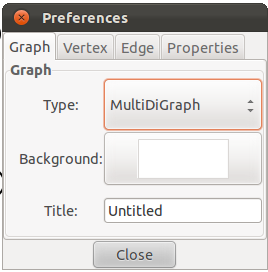
\includegraphics[width=7cm]{grape_global_preferences.png}
	\caption{Preferências}
	\label{img_global_preferences}
\end{figure}

\subsection{Menu View (Ver)}
\begin{figure}[htb]
    \centering
	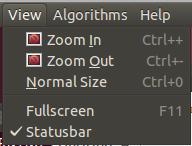
\includegraphics[width=6cm]{grape_menu_view.png}
	\caption{Menu ver}
	\label{img_menu_view}
\end{figure}

Esse nenu é utilizado para personalizar itens da interface do Grape, itens que devem ou não ser exibidos e opções de aproximar ou afastar o observador da área de pintura.

\begin{itemize}
    \item \textbf{Zoom In (Ampliar)}: Ação responsável por deixar a imagem da área de pintura mais próxima do observador.
    \item \textbf{Zoom Out (Afastar)}: Ação análoga a Ampliar, porém desta vez deixando a imagem da área de pintura mais distante do observador.
    \item \textbf{Normal Size (Tamanho normal)}: Restaura o tamanho da imagem da área de pintura para o tamanho normal.
    \item \textbf{Fullscreen (Tela cheia)}: Coloca ou remove a janela do Grape do modo tela cheia.
    \item \textbf{Statusbar (Barra de status)}: Mostra ou oculta a barra de status.
\end{itemize}

\subsection{Menu Algorithms (algoritmos)}
\begin{figure}[htb]
    \centering
	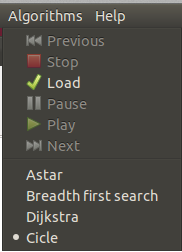
\includegraphics[width=6cm]{grape_menu_algorithms.png}
	\caption{Menu algoritmos}
	\label{img_menu_algorithms}
\end{figure}

Esse menu é utilizado para utilização dos algoritmos. Quando o Grape é carregado, ele preenche automaticamente este menu com os algorítimos presentes em seu determinado diretório. E as demais ações desse menu são para manipulação destes algorítimos.

\begin{itemize}
    \item \textbf{Previous (Anterior)}: Ação utilizada em casos de execução iterada, permite que o estado do algorítimo retroceda em uma iteração.
    \item \textbf{Stop (Parar)}: Interrompe a execução do algoritmo.
    \item \textbf{Load (Carregar)}: Carrega o algorítimo selecionado e o deixa pronto para iniciar a execução.
    \item \textbf{Pause (Pausa)}: Em caso de execução contínua esta ação irá passar para o modo iterativo, pausando a execução e aguardando pela próxima ação do usuário.
    \item \textbf{Play (Tocar)}: Inicia a execução contínua de um algorítimo que deve estar carregado com a ação Carregar.
    \item \textbf{Next (Próximo)}: Análogo à ação Anterior, porém agora, permite que o estado do algorítimo avance em uma iteração, para casos de execução iterada.
\end{itemize}

Os demais campos são os algorítimos de exemplo que foram carregados ao executar o Grape.

\subsection{Menu Help (Ajuda)}

Este menu apenas dirige o usuário para detalhes simples do Grape, na tela de about onde há um link para o código fonte e os créditos dos desenvolvedores.

\begin{figure}[htb]
    \centering
	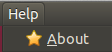
\includegraphics[width=3cm]{grape_menu_help.png}
	\caption{Menu Ajuda}
	\label{img_menu_help}
\end{figure}

\begin{figure}[H]
    \centering
	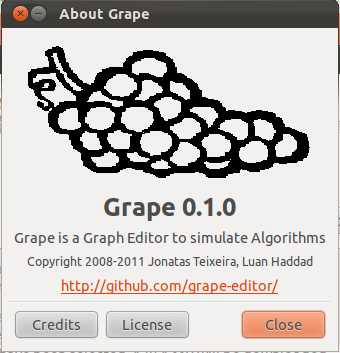
\includegraphics[width=8cm]{grape_about.png}
	\caption{Tela About}
	\label{img_about}
\end{figure}

\section{Atalhos e usabilidade}

O grape possui uma variedade de teclas de atalhos para acelerar o processo de criação e edição dos grafos, tais atalhos serão listados e brevemente descritos abaixo.

\begin{itemize}
    \item \textbf{Ctrl + N}: Abre um novo grafo em uma nova aba
    \item \textbf{Ctrl + O}: Abre diálogo para abrir um grafo
    \item \textbf{Ctrl + S}: Salvar grafo
    \item \textbf{Ctrl + Shift + S}: Salvar grafo especificando um local para ser salvo
    \item \textbf{Ctrl + Z}: Desfaz uma ação
    \item \textbf{Ctrl + Y}: Refaz uma ação
    \item \textbf{Ctrl + A}: Seleciona todos os vértices
    \item \textbf{V}: Inserir vértice
    \item \textbf{Shift + V}: Remover vértice
    \item \textbf{E}: Inserir aresta
    \item \textbf{Shift + E}: Remover aresta
    \item \textbf{Ctrl + +}: Aproximar
    \item \textbf{Ctrl + -}: Afastar
    \item \textbf{Ctrl + 0}: Voltar ao tamanho original
    \item \textbf{F11}: Exibir o grape um tela cheia
\end{itemize}

Setas direcionais: Selecionam o próximo vértice mais próximo do seguindo a direção da seta pressionada.

Uma forma alternativa de editar um vértice é simplesmente clicar com o botão direito do mouse sobre um vértice selecionado, E então será exibido um menu com opções de ações a serem efetuadas sobre este vértice, como mostrado na figura \ref{img_vertex_context_menu}.

\begin{figure}[htb]
    \centering
	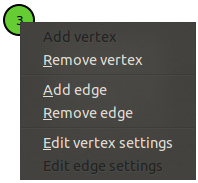
\includegraphics[width=6cm]{vertex_context_menu.png}
	\caption{Menu Vértice}
	\label{img_vertex_context_menu}
\end{figure}

Ao escolher editar as configurações de um vértice quer tenha sido pela barra de ferramentas ou pelo menu de propriedades do vértice será mostrado um diálogo que possibilita a personalização do vértice selecionado, onde há a possibilidade de editar o título do vértice, (o qual é exibido ná área de pintura), as coordenadas, a cor de preenchimento e da borda, o tamanho e a espessura da borda, também tem a possibilidade de listar todas as arestas que pertencem a esse vértice e de adicionar atributos personalizados. Por exemplo, na sessão Properties da edição de configurações de um vértice há um campo aonde existe uma tabela de atributos personalizados o qual possibilita ao usuário adicionar atributos quaisquer, que poderão ser acessados e/ou alterados pelos métodos set\_attribute e get\_attribute, no momento da execução dos algoritmos que serão vistos e explicados ao decorrer deste trabalho, os atributos personalizados funcionam como variáveis, ou seja, possuem um identificador e armazenam um valor, [identificador, valor].

Para que seja possível a edição de atributos personalizados das arestas é necessário que no menu de configurações do vértice “dono” da aresta, na aba edge uma aresta seja selecionada, e com o clique direito do mouse a opção de edição de aresta seja escolhida, só então abrirá uma nova tela para edições de atributos e propriedades da aresta escolhida.

\begin{figure}[htb]
    \centering
	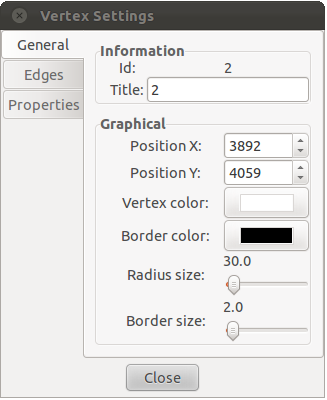
\includegraphics[width=7cm]{vertex_settings.png}
    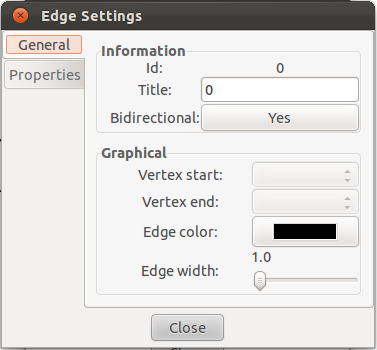
\includegraphics[width=7cm]{edge_settings.png}
	\caption{Configurações de vértice e aresta}
	\label{img_vertex_and_edges_settings}
\end{figure}

\chapter{algoritmos}

Implementamos no Grape um arcabouço para implementação de algoritmos, como ele foi implementado em python usando orientação a objetos seus algoritmos seguem a mesma linha. Neste capítulo iremos explicar algumas estruturas internas e algumas funções prontas para auxiliar a construção.

Os algoritmos podem ou não ser compilados para que sejam carregados, basta que eles estejam no diretório algorithms da raiz do Grape, antes dele ser executado, pois no momento da execução ele irá carregar dinamicamente todos os algoritmos que estiverem dentro daquele diretório e irá inserir cada um deles como entradas no menu Algoritmhs, como visto no Capítulo 5.

\section{Super Classe}

Todo algoritmo deve ser uma classe e estender uma super classe Algorithm para que então tenha acesso aos métodos de manipulação do grafo e da interface gráfica da representação do algoritmo.

\begin{python}
    from lib.algorithm import Algorithm
\end{python}

Métodos estendidos da super classe:

\begin{itemize}
    \item \textbf{check(object)}: Método que dará destaque a um objeto (vértice ou aresta) no próximo ciclo de execução.
    \item \textbf{uncheck(object)}: Analogamente ao método check, remove o destaque do objeto no próximo ciclo de execução.
    \item \textbf{show(object)}: Finaliza um ciclo de execução e mostra as alterações na área de pintura.
    \item \textbf{find(id)}: Busca um vértice por id no grafo e o retorna seu objeto.
    \item \textbf{set\_attribute(object, attribute, value)}: Cria ou altera um valor de um novo atributo  personalizado do objeto.
    \item \textbf{get\_attribute(object, attribute)}: Obtém o valor de um atributo personalizado criado com o set\_attribute, este atributo deverá ter sido criado usando o mesmo valor attribute no mesmo objeto object.
    \item \textbf{remove\_attribute(object, attribute)}: Remove um atributo attribute do objeto, após utilizar esse método o atributo deixará de existir, portanto não será mais acessível.
    \item \textbf{input\_box(descricao, texto, texto\_secundario)}: Cria uma caixa de texto, pedindo uma entrada para o usuário, e retorna um string contendo o valor de entrada fornecido pelo usuário.
\end{itemize}

Atributos estendidos da super classe:

\begin{itemize}
    \item \textbf{vertex\_list}: Lista com todos os vértices do grafo.
    \item \textbf{edge\_list}: Lista com todas as arestas do grafo.
\end{itemize}

Quando o algoritmo for executado a super classe vai chamar automaticamente o método run do algoritmo, logo este dever ser implementado no código do algoritmo de usuário. Também o nome do arquivo e da classe devem ser compatíveis: o nome do arquivo usar underline\_case e o da classe usar CamelCase. Por exemplo:

\begin{itemize}
    \item Arquivo: \textit{breadth\_first\_search.py}
    \item Classe: \textit{BreadthFirstSearch}
\end{itemize}

Ainda, no método construtor deverá ser feita a chamada ao construtor da super classe Algorithm, como visto no código abaixo:

\\
\begin{python}
class BreadthFirstSearch(Algorithm):
    def __init__(self, graph):
        Algorithm.__init__(self, graph)
\end{python}

Dentro desta classe podem ser criados quanto atributos e métodos forem necessários.

\section{Construindo Algoritmos}

Com o intuito de facilitar a construção de algoritmos usando o arcabouço do Grape fizemos um guia passo-a-passo:

Crie um arquivo python na pasta algorithms utilizando como nome o nome de seu algoritmo, procure sempre ser descritivos nos nomes, economizando abreviações. Vamos fazer um algoritmo de busca em profundidade (Depth-First Search), como descrito no livro \cite{cormen}, portanto usaremos o seguinte nome:

\$ touch algorithms/depth\_first\_search.py

Edite este arquivo usando seu editor favorito.

\$ vim algorithms/depth\_first\_search.py

Dentro dele crie uma classe utilizando o mesmo nome do arquivo, mas desta vez em CamelCase ao inves de underline\_case. Isto é muito importante pois internamente o Grape utiliza o padrão dos nomes para incluir seu algoritmo.

\\
\begin{python}
from lib.algorithm import Algorithm

class DepthFirstSearch(Algorithm):
    def __init__(self, graph):
         Algorithm.__init__(self, graph)
\end{python}

    Note que está parte do algoritmo é sempre igual. Nunca esqueça de estender da classe Algorithm e de definir o método construtor dessa forma, qualquer tentativa diferente disto implicará no não funcionamento de sua implementação. O método \_\_init\_\_  é o método construtor, podemos implementar mais coisas nele após a primeira linha, ele será executado automaticamente quando o usuário carrega o algoritmo na interface do Grape.

    O algoritmo de busca em profundidade parte de um vértice do grafo e tenta encontrar o destino expandindo cada aresta em forma de pilha, ou seja, a última aresta encontrada é a primeira a ser expandida. Para isso devemos saber o vértice origem e o vértice destino. Implementaremos no método construtor duas input\_box’s para que o usuário possa escolhe-los.

\\
\begin{python}
def __init__(self, graph):
        Algorithm.__init__(self, graph)
        # input box para capturarmos o vertice origem
        self.first_id = int(self.input_box('Escreva o numero do vertice origem', 'Origem'))
        # input box para capturarmos o vertice destino
        self.goal_id = int(self.input_box('Escreva o numero do vertice destino', 'Destino'))
\end{python}

Feito isto é hora de escrever o código do seu algoritmo, para isto, cria-se um método chamado run, o método run é executado automaticamente quando o usuário executa o algoritmo na interface do Grape. Portanto, devemos começar implementando o método run.

A primeira coisa que faremos é encontrar quais são os vértices baseando-se no que foi digitado pelo usuário:

\\
\begin{python}
    def run(self):
        first = self.find(self.first_id)
        goal = self.find(self.goal_id)
\end{python}

Tendo isso vamos criar nossa pilha de execução para adicionarmos as arestas e vértices a serem expandidos. Em python uma pilha é uma lista, apenas utilizada de forma correta.

\\
\begin{python}
        stack = [] # utlizaremos uma pilha para nossa busca em profundidade

        # adicionamos nosso inicio na pilha
        stack.append((first, None))
        # uma tupla (vertice, aresta). Como este e' o inicio nao
        # utilizamos nenhuma aresta para alcanca-lo
\end{python}

No início, nenhuma aresta foi visitada, portanto devemos marcar todas como “não visitadas”:

\\
\begin{python}
        # marcamos todas as arestas como nao visitados
        for e in self.edge_list:
            self.set_attribute(e, 'visited', 'no')
\end{python}

Começamos agora o algoritmo, ele deverá ser executando enquanto houverem elementos na pilha:

Capturamos o elemento no topo da pilha (em python o topo da pilha é o último elemento da lista, denotado por lista[-1]), marcamos como vistado e marcamos a aresta origem e o vértice para visualização:

\\
\begin{python}
        while len(stack) > 0:
            node = stack[-1]
            if node[1]:
                self.set_attribute(node[1], 'visited', 'yes')

            self.check(node[0])
            self.check(node[1])
            self.show()

            # Caso o vertice seja o destino, paramos por aqui o
            # algoritmo:
            if node[0].id == goal.id:
                rtn = node[0]
                break
\end{python}

    Caso contrário verificaremos se ainda há arestas a serem expandidas a partir deste vértice, isto se dá caso haja alguma aresta não visitada na vizinhança do vértice. Se não houver arestas a serem expandidas o vértice é removido da pilha e chamamos a próxima iteração do while.

\\
\begin{python}
            else:
                pop = True
                for edge in node[0].edge_list:
                    if self.get_attribute(edge, 'visited') == 'no':
                        pop = False
                        break

                if pop:
                    self.uncheck(node[0])
                    self.uncheck(node[1])
                    stack.pop()
                    continue
\end{python}

    Agora o algoritmo em si, na vizinhança do vértice atual procuraremos as arestas não visitadas e adicionaremos ela (juntamente com o vértice destino em questão) na pilha para ser expandida na próxima iteração.

\\
\begin{python}
            for edge in node[0].edge_list:
                if self.get_attribute(edge, 'visited') == 'no':
                    if edge.start == node[0]:
                        stack.append((edge.end, edge))
                    else:
                        stack.append((edge.start,edge))

\end{python}

% -----------------------------------------------------------------------
\chapter{Conclusão}
\label{sec:conclusao}

Com o Grape um ambiente de desenvolvimento é oferecido, aonde um aprendiz pode implementar através de uma linguagem de alto nível algoritmos à serem executados sobre uma estrutura de grafos. Partindo do premissa ideológica que uma lista é um tipo específico de árvore, e por sua vez uma árvore é um tipo específico de grafo, assim temos um grafo sendo a estrutura mais genérica para a representação em um ambiente de simulação iterativa de algoritmos

É esperado de uma ferramenta de apoio para o aprendizado de algoritmos que ela consiga de alguma maneira expor uma ambiente de depuração para que o aprendiz visualize o funcionamento do que está implementando, vendo possíveis erros à serem corrigidos ou até entendendo melhor o fluxo do algoritmo.

Como o Grape tem o mesmo propósito do Grafo, porém com outras representações e outra interface, podemos afirmar que a utilização de ferramentas como estas é muito proveitosa para aprendizado, tendo sido nós mesmos usuários deste ambiente.

Este trabalho conseguiu cumprir os objetivos traçados inicialmente para o Grape, fazendo o desenvolvimento técnico, teórico e conceitual de tudo que fora planejado.
% -----------------------------------------------------------------------

% -----------------------------------------------------------------------
\chapter{Trabalhos Futuros}
\label{sec:trabalhos_futuros}

Este trabalho deixa margem para variadas evoluções e em diversas vertentes.

A integração parcial com o NetworkX \cite{networkx} (Biblioteca de grafos para python) já foi implementada, porém a interface ainda não faz a comunicação necessária para exportar e importar arquivos nos formatos suportados pela biblioteca.

Além da interface gráfica GTK+ planejamos criar uma interface de linha de comando, tanto interpretativa quanto em modo batch, porque num ambiente de sala de aula onde o professor passa trabalhos de implementação é interessante que haja maneira de testar várias implementações com diferentes entradas de forma a comparar apenas o resultado sem ter o overhead de carregar toda a interface gráfica e manualmente executar cada uma das simulações para cada uma das entradas previstas.

Gostaríamos de publicar nosso simulador de grafos na \textit{GraphDrawing conference} \cite{graphdrawing}, uma conferência internacional de desenhos de grafos.

Como grafo é um modelo bastante genérico há a possibilidade de representar máquinas de estado em todas as suas variações.
% -----------------------------------------------------------------------

\bibliographystyle{acm}
\bibliography{tg.bib}

\end{document}

